
\subsubsection{Problem definition}

This calculation example, called Task~D\_THC~1, is done in the framework of the international DECOVALEX project. The model, which is described in the following, is a simplified 1~D benchmark test, which reproduces the processes in a generic repository in saturated crystalline rock where horizontal emplacement tunnels are backfilled with bentonite buffer material (Fig. \ref{fig81}, see chapter 8.1). The horizontal model begins at the left end with the heat source and includes bentonite and granite to the right of this source (Fig. \ref{fig91}). The model includes simulation of unsaturated flow, heat and mass transport coupled with a consideration of the reactions occurring (McDermott et al., 2007).

\subsubsection{Model set-up of the 2~D numerical model}

The material parameters for granite and bentonite buffer are given in Tab. \ref{tab81}, but the thermal conductivity of bentonite is set constant with a value of 1.3~W/(m$\cdot$K) and the heat capacity of bentonite is defined by the following function:
\begin{displaymath}
c\,=\,\left(1600\cdot\left(1.38\cdot T\,+\,732.5\right)
\,+\,1000\cdot\Phi\cdot S\cdot 4162\right)/p\,.
\end{displaymath}
The relationship between capillary pressure and saturation for both of granite and bentonite are depicted in Fig. \ref{fig83}. The relationship between relative permeability and saturation is described in Fig. \ref{fig84}. The model set-up including initial and boundary conditions is given in Fig. \ref{fig91}. The 1~D model begins from left end ($x=0.45$~m) to right end ($x=17.5$~m). It includes bentonite and granite and is discretised into 46 elements. The total simulation time is 1$\cdot$10$^6$ years.

\begin{figure}[htbp]
\centering
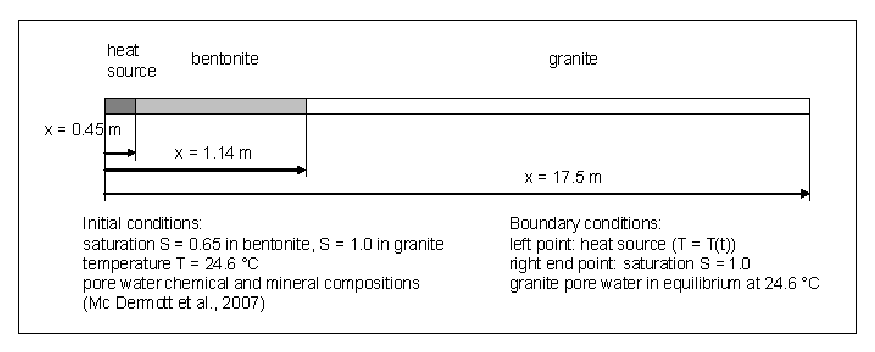
\includegraphics[width=0.9\textwidth]{THC/figures/fig91.eps}
\caption{Calculation model (1~D)}
\label{fig91}
\end{figure}

The mineral compositions of granite, bentonite and the related initial as well as equilibrated aqueous chemical compositions of porewater in granite and bentonite are given in McDermott et al. (2007). In granite the minerals Quartz, K-Feldspat, Plagioclase, Annite and Phlogopite are present. In bentonite also Quartz and K-Feldspat can be found, but also the minerals Na-Montmorillonite, Calcite, Dolomite and Pyrite. For mass transport, mass diffusion is included and the coefficients of mass diffusion for all ions and anions are assumed to be the same 1$\cdot$10$^{-9}$~m$^2$/s. The minerals are immobile. The geochemically balanced fluid and element concentrations (C, Ca, K, Na, Mg, Cl, Si, Al, S, Fe) are given in McDermott et al. (2007). The geochemical reactions considered in the simulation are aqueous and mineral-solution interactions. The chemical reactions in porewater are taken from the PHREEQC database. The temperature dependence of the reactions was regarded.

%\newpage

\subsubsection{Evaluation method}

The numerical results of the THC benchmark investigation are compared to those of TOUGH-REACT.

\subsubsection{Results}

The comparison of the results is presented in Fig. \ref{fig92} and Fig. \ref{fig93} for the 1000 year simulation case. Significant dissolution and precipitation is predicted at the contact between the different material groups of bentonite and granite. Both models predicted similar mineralogical alterations at the same location and to the same degree (McDermott et al., 2007)

\begin{figure}[htbp]
\centering
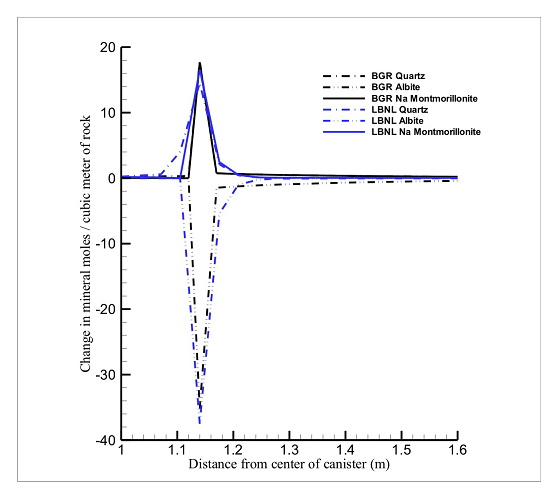
\includegraphics[width=0.7\textwidth]{THC/figures/fig92.eps}
\caption{Deposition of Quartz, Albite and Na-Montmorillonite after 1000 years of emplacement}
\label{fig92}
\end{figure}

\begin{figure}[htbp]
\centering
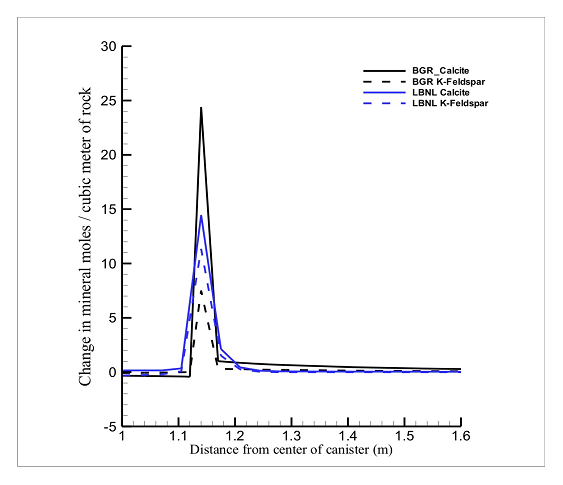
\includegraphics[width=0.7\textwidth]{THC/figures/fig93.eps}
\caption{Deposition of Calcite and K-Feldspat after 1000 years of emplacement}
\label{fig93}
\end{figure}



